%!TEX root = /home/renaud/Documents/EPL/tfe/latex/tfe.tex
\chapter{The "overturner" model}
\section{Mathematical model}
\subsection{Estimation of the parameter values}
\textcolor{red}{Vérifier que c'est bien les valeurs finales}
The numerical values used here are based on personal communications with \textit{E. Deleersnijder}.
The model for the idealized meridian velocity field in the Atlantic ocean will be complete once we have assigned plausible values to the parameters. For this purpose, some physical insight is needed. First, the Atlantic ocean extends approximately from $50\degree$ South to $60\degree$ North, hence over $\frac{11}{18}\pi$ radians. With the radius of the Earth estimated to $6\,371$ km, we get that $L$ must be close to $(\frac{11}{18}\pi) (6\,371) = 12\, 231$ km. Moreover, the mean depth of the Atlantic ocean is about $4$ km. Hence, we choose $L = 12\,000$ km and $H = 4$ km. In virtue of the properties of the streamfunction, the maximum $\Psi = \psi(y_0,z_0)$ of the meridian streamfunction is equal to the volume flow rate accross any curve connecting $(y_0,z_0)$ to a point on the boundary of the domain: it is thus a measure of the intensity of the meridian circulation. With an estimated rate of deep convection in the Atlantic ocean of about $20$ Sv and a mean width of about $5\,000$ km, this yields $\Psi = 4$ $\rm{m^2/s}$. Finally, we use $y_0 = 11\,000$ km and $z_0 = 3.5$ km based on qualitative inspection of the meridian streamfunction graph. Characteristic values $V$ and $W$ of the meridional and vertical speed are, in virtue of relations~\eqref{eq:u-psi} :
\begin{equation}\label{eq:VW}
	V = \frac{\Psi}{H} \quad \mbox{and} \quad W = \frac{\Psi}{L}.
\end{equation}
According to \textit{E. Deleersnijder} [personal communication], the characteristic time scale $T$ should be of the order of a few hundred years in order to be physically significant. It is expressed as
\begin{equation} \label{eq:T}
	T = \frac{L}{V} = \frac{H}{W} = \frac{LH}{\Psi} = 1.5\e{6} \mbox{ s} \approx 475.6 \mbox{ years},
\end{equation}
an acceptable value.

With those values of the parameters, the isolines of the adimensional streamfunction $\psi/\Psi$ are shown in figure~\ref{fig:psi_overturner}, and the meridional and vertical components of the velocity field are illustrated in figure~\ref{fig:vw_overturner}.
\begin{figure}[ht]
	\centering
	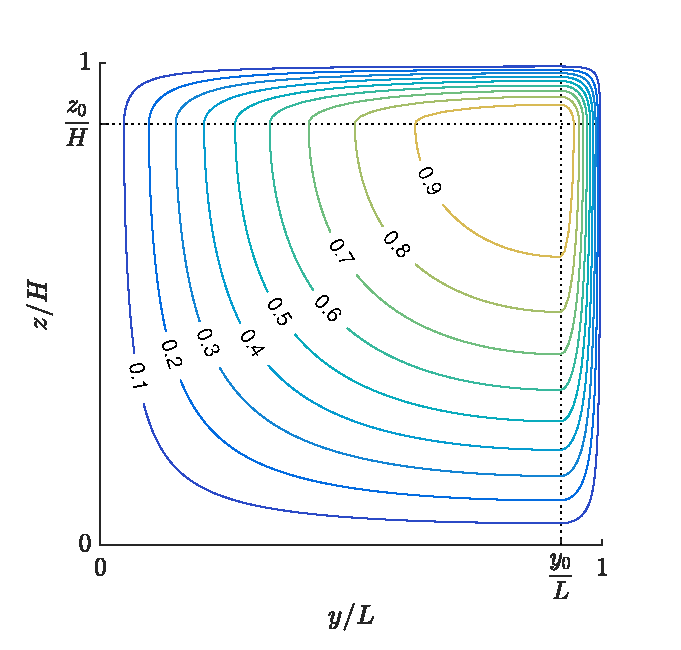
\includegraphics[width=.6\textwidth]{fig/overturner/psi.eps}
	\caption{Some isolines of the adimensional meridian streamfunction $\psi(y,z)/\Psi$, which are also streamlines of the idealised meridian circulation in the Atlantic ocean.}
	\label{fig:psi_overturner}
\end{figure}

\begin{figure}[ht]
	\centering
	\begin{subfigure}[t]{0.4\textwidth}
		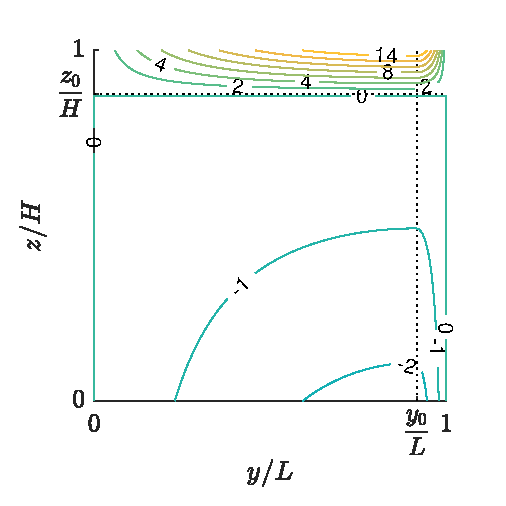
\includegraphics[width=\textwidth]{fig/overturner/V_samecaxis.eps}
		\caption{$v(y,z)$.}
		\label{fig:v_overturner}
	\end{subfigure}
	\begin{subfigure}[t]{0.4\textwidth}
		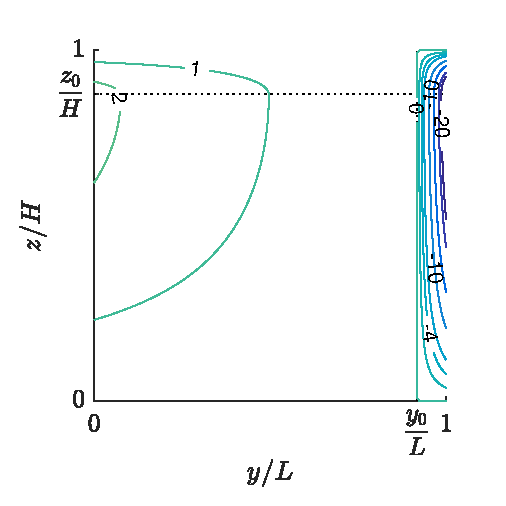
\includegraphics[width=\textwidth]{fig/overturner/W_samecaxis.eps}
		\caption{$w(y,z)$.}
		\label{fig:w_overturner}
	\end{subfigure}
	\begin{subfigure}[t]{0.1\textwidth}
		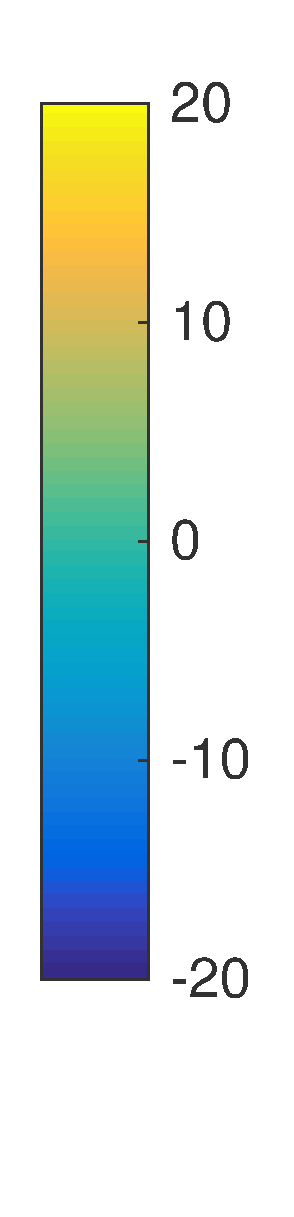
\includegraphics[height = 4\textwidth]{fig/overturner/colorbarVW.eps}
	\end{subfigure}
	\caption{Meridional and vertical components of the idealised velocity fields in the adimensional domain. Here, $y_0 = \frac{11}{12}L$ and $z_0 = \frac{7}{8}H$.}
	\label{fig:vw_overturner}
\end{figure}

\subsection{Injection of a passive tracer into the ocean} \label{sec:transport_overturner}
The fate of a passive tracer injected at location $(y_*,z_*)$ into the idealised Atlantic ocean depicted previously can be described by a differential problem on that tracer's concentration. The tracer could be any passive tracer whose concentration in the athmosphere is negligible, for example a dye or a set of seawater particles initially located at $(y_*,z_*)$. The concentration of the tracer $C(t,y,z)$ in the ocean obeys the following partial differential equation :
\begin{equation}\label{eq:C_PDE_vec}
	\frac{\partial C}{\partial t} = -\nabla \cdot \left(\b uC - \b K \nabla C\right),
\end{equation}
where $\b K$ is the \textit{diffusivity tensor}. Without loss of generality, we can assume $\b K$ to be symmetric. This is essentially because the impact of the anti-symmetric part of $\b K$, if any, may be viewed as additional advection. More details may be found in appendix A of \cite{deleersnijder2001concept}. Of course, the symmetric tensor $\b K$ must then be positive-definite in order to represent truly diffusive processes, namely phenoma which tend, at any time and location, to homogenise the concentration of any constituent. For our problem, we consider that $\b K$ has the form
\begin{equation} \label{eq:K}
	\b K(y,z) = \begin{pmatrix} K_h & 0 \\ 0 & K_v(y,z) \end{pmatrix},
\end{equation}
where $K_h$ is a positive constant and
\begin{equation} \label{eq:Kv}
	K_v(y,z) = \left\{ 
		\begin{array}{lrrr}
			K_{v_1} & \mbox{if} & y_0 \le y \le L, & 0 \le z \le H,\\
			K_{v_2} & \mbox{if} & 0 \le y < y_0, & 0 \le z < z_0,\\
			K_{v_3} & \mbox{if} & 0 \le y < y_0, & z_0 \le z \le H,
		\end{array}
	\right.
\end{equation}
with $K_{v_1}$, $K_{v_2}$ and $K_{v_3}$ positive constants. In the framework of the idealised model of the meridian circulation in the Atlantic ocean, \textit{E. Deleersnijder} [personal communication] proposes the values $K_h = 10^3$ $\rm{m^2/s}$, $K_{v_1} = 10^{-1}$ $\rm{m^2/s}$, $K_{v_2} = 10^{-4}$ $\rm{m^2/s}$ and $K_{v_3} = 10^{-3}$ $\rm{m^2/s}$. The relatively large value of $K_{v_1}$ allows to represent deep convection in the corresponding zone without having to implement a convective adjustment algorithm. The developped form of~\eqref{eq:C_PDE_vec} is then
\begin{equation}\label{eq:C_PDE_dev}
	\frac{\partial C}{\partial t} = -\frac{\partial}{\partial y}\left(vC - K_h\frac{\partial C}{\partial y}\right) -\frac{\partial}{\partial z}\left(wC - K_v(y,z)\frac{\partial C}{\partial z}\right).
\end{equation}
No-flux conditions are imposed at the boundaries \textcolor{red}{vérifier/discuter le flux nul à la surface}
\begin{equation}\label{eq:C_PDE_BC}
	\left. K_h\frac{\partial C}{\partial y} \right|_{y=0} = 0, \quad  \left. K_h\frac{\partial C}{\partial y} \right|_{y=L} = 0, \quad \left. K_v\frac{\partial C}{\partial z} \right|_{z=0} = 0, \quad \mbox{and} \quad \left. K_v\frac{\partial C}{\partial z} \right|_{z=H} = 0.
\end{equation}
The initial condition is
\begin{equation} \label{eq:C_PDE_CI}
	C(0,y,z) = \delta(y-y_*)\delta(z-z_*),
\end{equation}
where $\delta$ is the Dirac delta function, such that
\begin{equation}
	\int_0^L \int_0^H C(0,y,z) \rm dy \rm dz = 1.
\end{equation}

In order to get a formulation of the problem using as few independent parameters as possible, it is interesting to consider the adimensional formulation. Such a scaling is particularly interesting for sensitivity analysis. The adimensional independent variables are
\begin{equation}
	t' = \frac{t}{T} = \frac{t\Psi}{LH}, \quad y' = \frac{y}{L} \quad \mbox{and} \quad z' = \frac{z}{H},   	
\end{equation}
where $T$ is the time scale introduced in~\eqref{eq:T}. The adimensional hydrodynamic variables are:
\begin{equation}
	\psi' = \frac{\psi}{\Psi}, \quad v' = \frac{v}{V} = \frac{vH}{\Psi}, \quad \mbox{and} \quad w' = \frac{w}{W} = \frac{wL}{\Psi},
\end{equation}
where $V$ and $W$ are the velocity scales introduced in~\eqref{eq:VW}. The adimensional concentration is
\begin{equation}
	C' = \frac{C}{C_r}, 	
\end{equation}
where $C_r$ is a characteristic value of the concentration. We will see shortly that there is no needed to assign a particular value to $C_r$. The adimensional form of equation~\eqref{eq:C_PDE_dev} is then
\begin{equation}\label{eq:PDE_adim}
	\frac{\partial C'}{\partial t'} = -\frac{\partial}{\partial y'}\left(v'C' - \frac{1}{Pe_h}\frac{\partial C'}{\partial y'}\right) -\frac{\partial}{\partial z'}\left(w'C' - \frac{1}{Pe_v(y,z)}\frac{\partial C'}{\partial z'}\right),
\end{equation}
where
\begin{equation}
	Pe_h = \frac{\Psi L}{K_h H} \quad \mbox{and} \quad Pe_v(y,z) = \frac{\Psi H}{K_v(y,z)L}
\end{equation}
are the horizontal and vertical Péclet numbers. They correspond to the ratio between the characteristic advective and diffusive velocity scales. Indeed, the horizontal and vertical diffusive velocity scales $V_{d}$ and $W_{d}$ are 
\begin{equation}
	V_{d} = \frac{K_h}{L} \quad \mbox{and} \quad W_{d}(y,z) = \frac{K_v(y,z)}{H}.
\end{equation}
There are three different vertical diffusive velocity scale depending on which zone of the ocean we consider \textcolor{red}{Donner des noms aux zones dans le chap 1 : 1 = ?, 2 = "Deep convection" et 3 = "surface flow"}. The advective velocity scales $V$ and $W$ have already been introduced in~\eqref{eq:VW}. The Péclet numbers may then be rewritten as
\begin{equation}
	Pe_h = \frac{V}{V_{d}} = 12, 
\end{equation}
and
\begin{equation}
	Pe_{v}(y,z) =  \frac{W}{W_{d}(y,z)}=  \left\{
	\begin{array}{lrrr}
			Pe_{v_1} = 1.33\e{-2} & \mbox{if} & y_0 \le y \le L, & 0 \le z \le H,\\
			Pe_{v_2} = 13.3 & \mbox{if} & 0 \le y < y_0, & 0 \le z < z_0,\\
			Pe_{v_3} = 1.33 & \mbox{if} & 0 \le y < y_0, & z_0 \le z \le H.
	\end{array}
	\right.
\end{equation}
This shows that the advective and diffusive processes are of equal importance in the dynamics of our model, excepted in the zone of deep convection where the vertical diffusion dominates the vertical convection. This is because we have chosen to represent deep convection via a heavy vertical mixing in that zone. 